\documentclass{article}
\usepackage[paperwidth=20cm,paperheight=12cm,margin=0.3cm]{geometry}
\pagestyle{empty}
\usepackage{tikz}
\usetikzlibrary{arrows.meta, positioning, calc, fit, backgrounds, decorations.pathreplacing}

\begin{document}
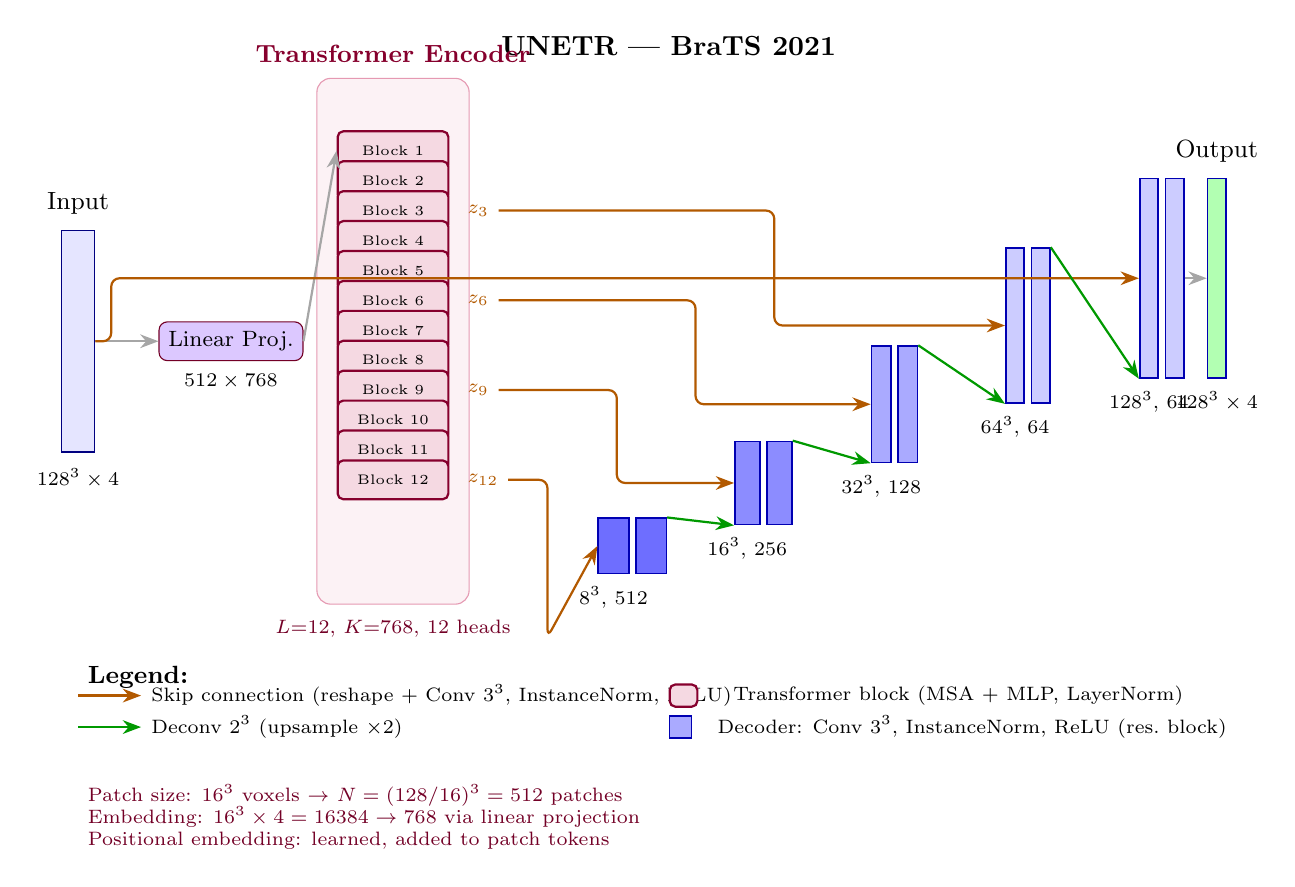
\begin{tikzpicture}[
    >=Stealth,
    font=\footnotesize,
    block/.style={draw=blue!70!black, line width=0.6pt, fill=#1, minimum width=5pt},
    tblock/.style={draw=purple!70!black, line width=0.8pt, fill=purple!15,
                   minimum width=18pt, minimum height=14pt, rounded corners=2pt},
    arrow/.style={->, thick, draw=gray!70},
    skip/.style={->, thick, draw=orange!70!black},
    up/.style={->, thick, draw=green!60!black},
]

% === Color definitions ===
\definecolor{patch}{RGB}{220,200,255}    % light purple for patch embedding
\definecolor{trans}{RGB}{240,220,255}    % transformer blocks
\definecolor{dec1}{RGB}{204,204,255}     % decoder blues (lightest)
\definecolor{dec2}{RGB}{170,170,255}
\definecolor{dec3}{RGB}{140,140,255}
\definecolor{dec4}{RGB}{110,110,255}     % darkest

% === Title ===
\node[font=\normalsize\bfseries, anchor=south] at (7.5, 5.5) {UNETR --- BraTS 2021};

% === Input ===
\node[block=blue!10, minimum height=80pt, minimum width=12pt, draw=blue!50!black] (input) at (0, 2) {};
\node[below=2pt of input, font=\scriptsize, align=center] {$128^3 \times 4$};
\node[above=2pt of input, font=\small] {Input};

% === Patch Embedding ===
\node[draw=purple!60!black, fill=patch, minimum height=14pt, minimum width=50pt,
      rounded corners=3pt, right=0.8cm of input] (pembed) {Linear Proj.};
\node[below=1pt of pembed, font=\scriptsize] {$512 \times 768$};

% === Transformer Encoder (12 blocks, show key extraction points) ===
% Draw transformer as a vertical stack with extraction arrows
\def\tstart{4.0}
\def\tspacing{0.38}

% Background box for transformer
\begin{scope}[on background layer]
\node[draw=purple!40, fill=purple!5, rounded corners=5pt,
      minimum width=55pt, minimum height=190pt] (tbox) at (\tstart, 2) {};
\end{scope}
\node[above=2pt of tbox, font=\small\bfseries, text=purple!70!black] {Transformer Encoder};
\node[below=2pt of tbox, font=\scriptsize, text=purple!60!black] {$L{=}12$, $K{=}768$, 12 heads};

% Transformer layers (simplified as stacked blocks)
\foreach \i [evaluate=\i as \y using {2 + 2.8 - \i*\tspacing}] in {1,...,12} {
    \node[tblock, minimum width=40pt] (t\i) at (\tstart, \y) {\tiny Block \i};
}

% Extraction indicators
\foreach \i/\lab in {3/$z_3$, 6/$z_6$, 9/$z_9$, 12/$z_{12}$} {
    \node[right=3pt of t\i, font=\scriptsize\bfseries, text=orange!70!black] (ext\i) {\lab};
}

% === Decoder Path (right side, ascending) ===
% z12 → bottleneck path
\node[block=dec4, minimum height=20pt, minimum width=11pt] (b1) at (6.8, -0.6) {};
\node[block=dec4, minimum height=20pt, minimum width=11pt, right=2pt of b1] (b2) {};
\node[below=1pt of b1, font=\scriptsize, anchor=north] {$8^3$, 512};

% z9 path
\node[block=dec3, minimum height=30pt, minimum width=9pt] (d9a) at (8.5, 0.2) {};
\node[block=dec3, minimum height=30pt, minimum width=9pt, right=2pt of d9a] (d9b) {};
\node[below=1pt of d9a, font=\scriptsize, anchor=north] {$16^3$, 256};

% z6 path
\node[block=dec2, minimum height=42pt, minimum width=7pt] (d6a) at (10.2, 1.2) {};
\node[block=dec2, minimum height=42pt, minimum width=7pt, right=2pt of d6a] (d6b) {};
\node[below=1pt of d6a, font=\scriptsize, anchor=north] {$32^3$, 128};

% z3 path
\node[block=dec1, minimum height=56pt, minimum width=5pt] (d3a) at (11.9, 2.2) {};
\node[block=dec1, minimum height=56pt, minimum width=5pt, right=2pt of d3a] (d3b) {};
\node[below=1pt of d3a, font=\scriptsize, anchor=north] {$64^3$, 64};

% Final resolution (input skip)
\node[block=blue!20, minimum height=72pt, minimum width=5pt] (d0a) at (13.6, 2.8) {};
\node[block=blue!20, minimum height=72pt, minimum width=5pt, right=2pt of d0a] (d0b) {};
\node[below=1pt of d0a, font=\scriptsize, anchor=north] {$128^3$, 64};

% Output conv
\node[block=green!30, minimum height=72pt, minimum width=3pt, right=8pt of d0b] (out) {};
\node[above=2pt of out, font=\small] {Output};
\node[below=1pt of out, font=\scriptsize, anchor=north] {$128^3 \times 4$};

% === Connections ===
% Input to patch embedding
\draw[arrow] (input.east) -- (pembed.west);

% Patch embedding to transformer
\draw[arrow] (pembed.east) -- (t1.west);

% Skip connections from transformer to decoder (reshape + project)
\draw[skip, rounded corners=3pt] (ext12.east) -| ++(0.5, -2.0) -- (b1.west);
\draw[skip, rounded corners=3pt] (ext9.east) -- ++(1.5, 0) |- (d9a.west);
\draw[skip, rounded corners=3pt] (ext6.east) -- ++(2.5, 0) |- (d6a.west);
\draw[skip, rounded corners=3pt] (ext3.east) -- ++(3.5, 0) |- (d3a.west);

% Input skip to final decoder stage
\draw[skip, rounded corners=3pt] (input.east) -- ++(0.2, 0) |- (d0a.west);

% Upsampling between decoder stages
\draw[up] (b2.north east) -- (d9a.south west);
\draw[up] (d9b.north east) -- (d6a.south west);
\draw[up] (d6b.north east) -- (d3a.south west);
\draw[up] (d3b.north east) -- (d0a.south west);

% Output arrow
\draw[arrow] (d0b.east) -- (out.west);

% === Legend ===
\node[anchor=north west, font=\small\bfseries] at (0, -2.0) {Legend:};
\draw[skip] (0, -2.5) -- ++(0.8, 0) node[right, font=\scriptsize] {Skip connection (reshape $+$ Conv $3^3$, InstanceNorm, ReLU)};
\draw[up] (0, -2.9) -- ++(0.8, 0) node[right, font=\scriptsize] {Deconv $2^3$ (upsample $\times 2$)};

\node[tblock, minimum width=10pt, minimum height=8pt, anchor=west] at (7.5, -2.5) {};
\node[right, font=\scriptsize] at (8.2, -2.5) {Transformer block (MSA $+$ MLP, LayerNorm)};

\node[block=dec2, minimum height=8pt, minimum width=8pt, anchor=west] at (7.5, -2.9) {};
\node[right, font=\scriptsize] at (8.0, -2.9) {Decoder: Conv $3^3$, InstanceNorm, ReLU (res.\ block)};

% Patch info annotation
\node[font=\scriptsize, text=purple!60!black, align=left, anchor=north west] at (0, -3.5)
    {Patch size: $16^3$ voxels $\rightarrow$ $N = (128/16)^3 = 512$ patches\\
     Embedding: $16^3 \times 4 = 16384 \rightarrow 768$ via linear projection\\
     Positional embedding: learned, added to patch tokens};

\end{tikzpicture}
\end{document}
